% GNUPLOT: LaTeX picture with Postscript
\begingroup
  \makeatletter
  \providecommand\color[2][]{%
    \GenericError{(gnuplot) \space\space\space\@spaces}{%
      Package color not loaded in conjunction with
      terminal option `colourtext'%
    }{See the gnuplot documentation for explanation.%
    }{Either use 'blacktext' in gnuplot or load the package
      color.sty in LaTeX.}%
    \renewcommand\color[2][]{}%
  }%
  \providecommand\includegraphics[2][]{%
    \GenericError{(gnuplot) \space\space\space\@spaces}{%
      Package graphicx or graphics not loaded%
    }{See the gnuplot documentation for explanation.%
    }{The gnuplot epslatex terminal needs graphicx.sty or graphics.sty.}%
    \renewcommand\includegraphics[2][]{}%
  }%
  \providecommand\rotatebox[2]{#2}%
  \@ifundefined{ifGPcolor}{%
    \newif\ifGPcolor
    \GPcolorfalse
  }{}%
  \@ifundefined{ifGPblacktext}{%
    \newif\ifGPblacktext
    \GPblacktexttrue
  }{}%
  % define a \g@addto@macro without @ in the name:
  \let\gplgaddtomacro\g@addto@macro
  % define empty templates for all commands taking text:
  \gdef\gplfronttext{}%
  \gdef\gplfronttext{}%
  \makeatother
  \ifGPblacktext
    % no textcolor at all
    \def\colorrgb#1{}%
    \def\colorgray#1{}%
  \else
    % gray or color?
    \ifGPcolor
      \def\colorrgb#1{\color[rgb]{#1}}%
      \def\colorgray#1{\color[gray]{#1}}%
      \expandafter\def\csname LTw\endcsname{\color{white}}%
      \expandafter\def\csname LTb\endcsname{\color{black}}%
      \expandafter\def\csname LTa\endcsname{\color{black}}%
      \expandafter\def\csname LT0\endcsname{\color[rgb]{1,0,0}}%
      \expandafter\def\csname LT1\endcsname{\color[rgb]{0,1,0}}%
      \expandafter\def\csname LT2\endcsname{\color[rgb]{0,0,1}}%
      \expandafter\def\csname LT3\endcsname{\color[rgb]{1,0,1}}%
      \expandafter\def\csname LT4\endcsname{\color[rgb]{0,1,1}}%
      \expandafter\def\csname LT5\endcsname{\color[rgb]{1,1,0}}%
      \expandafter\def\csname LT6\endcsname{\color[rgb]{0,0,0}}%
      \expandafter\def\csname LT7\endcsname{\color[rgb]{1,0.3,0}}%
      \expandafter\def\csname LT8\endcsname{\color[rgb]{0.5,0.5,0.5}}%
    \else
      % gray
      \def\colorrgb#1{\color{black}}%
      \def\colorgray#1{\color[gray]{#1}}%
      \expandafter\def\csname LTw\endcsname{\color{white}}%
      \expandafter\def\csname LTb\endcsname{\color{black}}%
      \expandafter\def\csname LTa\endcsname{\color{black}}%
      \expandafter\def\csname LT0\endcsname{\color{black}}%
      \expandafter\def\csname LT1\endcsname{\color{black}}%
      \expandafter\def\csname LT2\endcsname{\color{black}}%
      \expandafter\def\csname LT3\endcsname{\color{black}}%
      \expandafter\def\csname LT4\endcsname{\color{black}}%
      \expandafter\def\csname LT5\endcsname{\color{black}}%
      \expandafter\def\csname LT6\endcsname{\color{black}}%
      \expandafter\def\csname LT7\endcsname{\color{black}}%
      \expandafter\def\csname LT8\endcsname{\color{black}}%
    \fi
  \fi
  \setlength{\unitlength}{0.0500bp}%
  \begin{picture}(8000.00,10000.00)%
    \gplgaddtomacro\gplfronttext{%
      \colorrgb{0.00,0.00,0.00}%
      \put(716,10200){\makebox(0,0){\strut{}\small $\sigma_R = 0.01$}}%
      \colorrgb{0.00,0.00,0.00}%
      \put(2029,10200){\makebox(0,0){\strut{}\small $\sigma_R = 0.03$}}%
      \colorrgb{0.00,0.00,0.00}%
      \put(3343,10200){\makebox(0,0){\strut{}\small $\sigma_R = 0.05$}}%
      \colorrgb{0.00,0.00,0.00}%
      \put(4656,10200){\makebox(0,0){\strut{}\small $\sigma_R = 0.10$}}%
      \colorrgb{0.00,0.00,0.00}%
      \put(5969,10200){\makebox(0,0){\strut{}\small $\sigma_R = 0.20$ [m]}}%
    }%
    \gplgaddtomacro\gplfronttext{%
      \colorrgb{0.00,0.00,0.00}%
      \put(-700,9400){\rotatebox{90}{\makebox(0,0){\strut{}\small PLICP}}}%
      \put(-700,8300){\rotatebox{90}{\makebox(0,0){\strut{}\small NDT}}}%
      \put(-700,7200){\rotatebox{90}{\makebox(0,0){\strut{}\small FastGICP}}}%
      \put(-700,6100){\rotatebox{90}{\makebox(0,0){\strut{}\small FastVGICP}}}%
      \put(-700,5000){\rotatebox{90}{\makebox(0,0){\strut{}\small NDT-PSO}}}%
      \put(-700,3900){\rotatebox{90}{\makebox(0,0){\strut{}\small TEASER}}}%
      \put(-700,2800){\rotatebox{90}{\makebox(0,0){\strut{}\small \texttt{x1}}}}%
      \put(-700,1700){\rotatebox{90}{\makebox(0,0){\strut{}\small \texttt{uf}}}}%
      \put(-700,600){\rotatebox{90}{\makebox(0,0){\strut{}\small \texttt{fm}}}}%
    }%
    \gplgaddtomacro\gplfronttext{%
      \colorrgb{0.00,0.00,0.00}%
      \put(7800,100){\makebox(0,0)[l]{\strut{}$0.0$}}%
      \colorrgb{0.00,0.00,0.00}%
      \put(7800,1516){\makebox(0,0)[l]{\strut{}$0.02$}}%
      \colorrgb{0.00,0.00,0.00}%
      \put(7800,2933){\makebox(0,0)[l]{\strut{}$0.04$}}%
      \colorrgb{0.00,0.00,0.00}%
      \put(7800,4349){\makebox(0,0)[l]{\strut{}$0.06$}}%
      \colorrgb{0.00,0.00,0.00}%
      \put(7800,5766){\makebox(0,0)[l]{\strut{}$0.08$}}%
      \colorrgb{0.00,0.00,0.00}%
      \put(7800,7182){\makebox(0,0)[l]{\strut{}$0.10$}}%
      \colorrgb{0.00,0.00,0.00}%
      \put(7800,8599){\makebox(0,0)[l]{\strut{}$0.12$}}%
      \colorrgb{0.00,0.00,0.00}%
      \put(7800,9899){\makebox(0,0)[l]{\strut{}$> e_{\sigma_{\bm{M}}}^{\text{avg}} = 0.138$}}%

      \put(-200,5000) {\rotatebox{90}{\makebox(0,0){\strut{}$\|\Delta \hat{\bm{l}}\|_2 \in [0, \sqrt{2} \cdot \overline{\delta}_{xy}]$}}}%
      \put(3343,-156){\makebox(0,0){\strut{}$\Delta\hat{\theta} \in [-\overline{\delta}_\theta, +\overline{\delta}_\theta]$}}
    }%
    \put(0,0){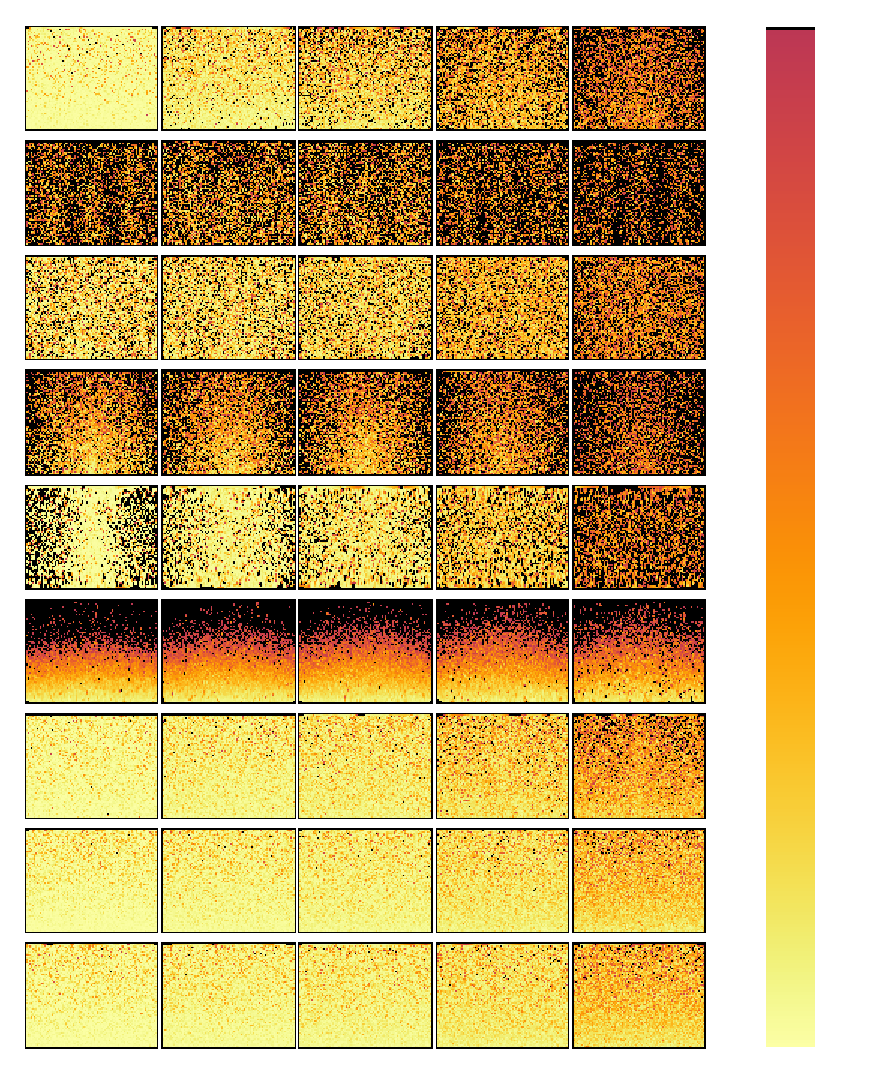
\includegraphics{./figures/parts/02/chapters/04/sections/05/caer_style_pose_errors_sm0}}%
    \gplfronttext
  \end{picture}%
\endgroup
